

\documentclass[11pt,a4paper,twoside]{article}

\usepackage[utf8]{inputenc}
\usepackage[english]{babel} 
\usepackage{notoccite}
\usepackage[skip=0.5\baselineskip]{caption}
\hyphenation{GTKWave}
\usepackage{listings}
\usepackage[all]{nowidow}
\usepackage{amsmath} %Matrix package
\usepackage{csvsimple} %csv reading package
\usepackage{authblk} %author information
\usepackage{caption}
\usepackage{multicol}
\usepackage{fancyhdr}
\usepackage{booktabs}
\usepackage{float}
\usepackage{multirow}
\usepackage[justification=centering]{caption}
\usepackage{siunitx}
\usepackage[english]{babel}
\usepackage{graphicx}
\usepackage{amsmath,amssymb}
\usepackage{lmodern}
\usepackage{iftex}
\ifPDFTeX
  \usepackage[T1]{fontenc}
  \usepackage[utf8]{inputenc}
  \usepackage{textcomp} % provide euro and other symbols  
\usepackage{titlesec}
\restylefloat{table}


\usepackage{graphicx}
\graphicspath{{./}{../../figlib/}{../mat/}{../sim/}}
\def\FontLn{% 16 pt normal
  \usefont{T1}{phv}{m}{n}\fontsize{16pt}{16pt}\selectfont}
\def\FontLb{% 16 pt bold
  \usefont{T1}{phv}{b}{n}\fontsize{16pt}{16pt}\selectfont}
\def\FontMn{% 14 pt normal
  \usefont{T1}{phv}{m}{n}\fontsize{14pt}{14pt}\selectfont}
\def\FontMb{% 14 pt bold
  \usefont{T1}{phv}{b}{n}\fontsize{14pt}{14pt}\selectfont}
\def\FontSn{% 12 pt normal
  \usefont{T1}{phv}{m}{n}\fontsize{12pt}{12pt}\selectfont}

\renewcommand{\rmdefault}{phv}
\renewcommand{\sfdefault}{phv}
\usepackage{geometry}	
\geometry{verbose,tmargin=2.5cm,bmargin=2.5cm,lmargin=2.5cm,rmargin=2.5cm}

%\usepackage{setspace}
%\renewcommand{\baselinestretch}{1.5}

\usepackage[pdftex]{hyperref} % enhance documents that are to be
                              % output as HTML and PDF
\hypersetup{colorlinks,       % color text of links and anchors,
                              % eliminates borders around links
%            linkcolor=red,    % color for normal internal links
            linkcolor=black,  % color for normal internal links
            anchorcolor=black,% color for anchor text
%            citecolor=green,  % color for bibliographical citations
            citecolor=black,  % color for bibliographical citations
%            filecolor=magenta,% color for URLs which open local files
            filecolor=black,  % color for URLs which open local files
%            menucolor=red,    % color for Acrobat menu items
            menucolor=black,  % color for Acrobat menu items
%            pagecolor=red,    % color for links to other pages
            pagecolor=black,  % color for links to other pages
%            urlcolor=cyan,    % color for linked URLs
            urlcolor=black,   % color for linked URLs
	          bookmarks=true,         % create PDF bookmarks
	          bookmarksopen=false,    % don't expand bookmarks
	          bookmarksnumbered=true, % number bookmarks
	          pdftitle={report},
            pdfauthor={Andre C. Marta},
%            pdfsubject={Thesis Title},
%            pdfkeywords={Thesis Keywords},
            pdfstartview=FitV,
            pdfdisplaydoctitle=true}

\usepackage[numbers,sort&compress]{natbib} % <<<<< References in numbered list [1],[2],...
\usepackage{subcaption} 
\usepackage{mdframed}

%%%%%%%%%%%%%%%%%%%%%%%%%%%%%%%%%%%%%%%%%%%%%%%%%%%%%%%%%%%%%%%%%%%%%%%%
%     Begin Document                                                   %
%%%%%%%%%%%%%%%%%%%%%%%%%%%%%%%%%%%%%%%%%%%%%%%%%%%%%%%%%%%%%%%%%%%%%%%%


\begin{document}

% Set plain page style (no headers, footer with centered page number)
\pagestyle{plain}

% Set roman numbering (i,ii,...) before the start of chapters
%\pagenumbering{roman}

% ----------------------------------------------------------------------
%  Cover page
% ----------------------------------------------------------------------
\begin{titlepage}
%%%%%%%%%%%%%%%%%%%%%%%%%%%%%%%%%%%%%%%%%%%%%%%%%%%%%%%%%%%%%%%%%%%%%%%%
%                                                                      %
%     File: frontvover.tex                                      %
%     Tex Master: report.tex                                           %
%                                                                      %
%     Author: Group 41                                           %
%     Last modified :  3 Mar 2021                                      %
%                                                                      %
%%%%%%%%%%%%%%%%%%%%%%%%%%%%%%%%%%%%%%%%%%%%%%%%%%%%%%%%%%%%%%%%%%%%%%%%

\thispagestyle {empty}

% IST Logo - Signature A
% parameters: bb=llx lly urx ury (bounding box), width=h_length, height=v_length, angle=angle, scale=factor, clip=true/false, draft=true/false. 
\includegraphics[bb=9.5cm 11cm 0cm 0cm,scale=0.29]{IST_A_CMYK_POS}

\begin{center}
%

\vspace{1.0cm}


% Title, author and degree
\vspace{1cm}
{\FontLb Circuit Theory and Electronics Fundamentals} \\ % <<<<< EDIT TITLE
\vspace{1cm}
{\FontSn Aerospace Engineering, Técnico, University of Lisbon} \\ % <<<<< EDIT COURSE
\vspace{1cm}
{\FontSn T1 Laboratory Report} \\
\vspace{1cm}
{\FontSn March 6, 2021} \\ % <<<<< EDIT DATE (corresponds to date of oral examination)
\vspace{1cm}
\author{Duarte Brito 96373 \and Henrique Caraça 96393 \and Nuno Ribeiro 96459}
\end{center}


\end{titlepage}

% ----------------------------------------------------------------------
% Dedication page (optional)
% ----------------------------------------------------------------------
%\input{dedication} 
%\cleardoublepage

% ----------------------------------------------------------------------
%  Acknowledgments (optional)
% ----------------------------------------------------------------------
%\input{acknowledgements}
%\cleardoublepage

% ----------------------------------------------------------------------
%  Abstract (both in English and Portuguese)
% ----------------------------------------------------------------------
%\input{resumo} 
%\cleardoublepage

%\input{abstract} 

% ----------------------------------------------------------------------
%  Table of contents, list of tables, list of figures and nomenclature
% ----------------------------------------------------------------------

%\pagestyle{fancy}
%\rhead{\leftmark}
%\lhead{Movimento Giroscópio}


% Table of contents
%
\tableofcontents

% List of tables
%\addcontentsline{toc}{section}{\listtablename}
%\listoftables
%\cleardoublepage 

% List of figures
%\addcontentsline{toc}{section}{\listfigurename}
%\listoffigures
%\cleardoublepage 

% Set arabic numbering (1,2,...) after preface
%
%\setcounter{page}{1}
%\pagenumbering{arabic}

% ----------------------------------------------------------------------
%  Body
% ----------------------------------------------------------------------

\section{Introduction}
\label{sec:introduction}

\indent

% state the learning objective 
The objective of this laboratory assignment is to make a Bandpass filter using an OP-AMP.

The equivalent circuit can be seen in Figure~\ref{fig:circuit}. 

This circuit is made up of an amplifier (an OP-AMP and resistors $R_3$ and $R_4$), a high pass filter (the left part, that is $C_1$ and $R_1$),  and a low pass filter (the right part, that is $R_2$ and $C_2$) .

In Section~\ref{sec:simulation analysis}, the circuit is analysed by
means of a ngspice simulation. In Section~\ref{sec:theoretical analysis}, a theoretical analysis of the circuit is
presented. The results are then compared in Section~\ref{sec:theoretical analysis}. The conclusions of this study are outlined in Section~\ref{sec:conclusion}.



\begin{figure}[h!] \centering
	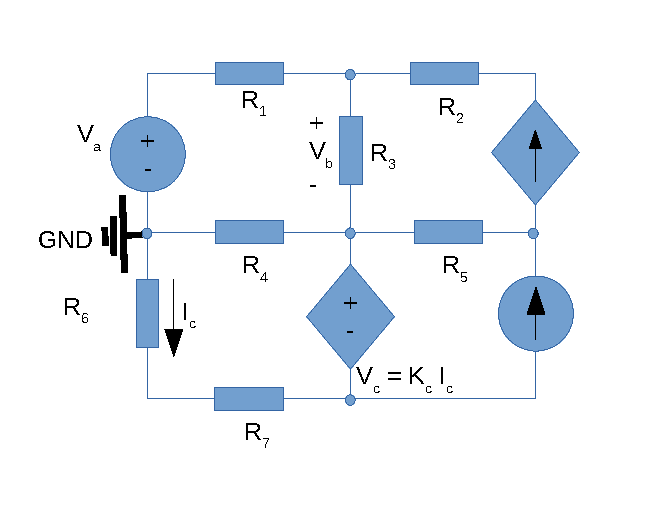
\includegraphics[width=0.6\linewidth]{circ.pdf}
	\caption{Used Circuit.}
	\label{fig:circuit}
\end{figure}






\section{Simulation Analysis}
\label{sec:simulation}

\subsection{Operating Point Analysis}

Table~\ref{tab:op} shows the simulated operating point results for the circuit
under analysis. Compared to the theoretical analysis results, one notices the
following differences: describe and explain the differences.

\begin{table}[h]
  \centering
  \begin{tabular}{|l|r|}
    \hline    
    {\bf Name} & {\bf Value [A or V]} \\ \hline
    @gb[i] & -2.47520e-04\\ \hline
@id[current] & 1.005321e-03\\ \hline
@r1[i] & 2.364560e-04\\ \hline
@r2[i] & -2.47520e-04\\ \hline
@r3[i] & -1.10640e-05\\ \hline
@r4[i] & 1.201119e-03\\ \hline
@r5[i] & -1.25284e-03\\ \hline
@r6[i] & 9.646630e-04\\ \hline
@r7[i] & 9.646630e-04\\ \hline
v(1) & 5.076387e+00\\ \hline
v(2) & 4.828240e+00\\ \hline
v(3) & 4.317615e+00\\ \hline
v(4) & 4.862301e+00\\ \hline
v(5) & 8.665725e+00\\ \hline
v(6) & -1.94693e+00\\ \hline
v(7) & -2.95363e+00\\ \hline
v(9) & -1.94693e+00\\ \hline

  \end{tabular}
  \caption{Operating point. A variable preceded by @ is of type {\em current}
    and expressed in Ampere; other variables are of type {\it voltage} and expressed in
    Volt.}
  \label{tab:op}
\end{table}

\lipsum[1-1]


\subsection{Transient Analysis}

Figure~\ref{fig:trans} shows the simulated transient analysis results for the
circuit under analysis. Compared to the theoretical analysis results, one
notices the following differences: describe and explain the differences.

\begin{figure}[h] \centering
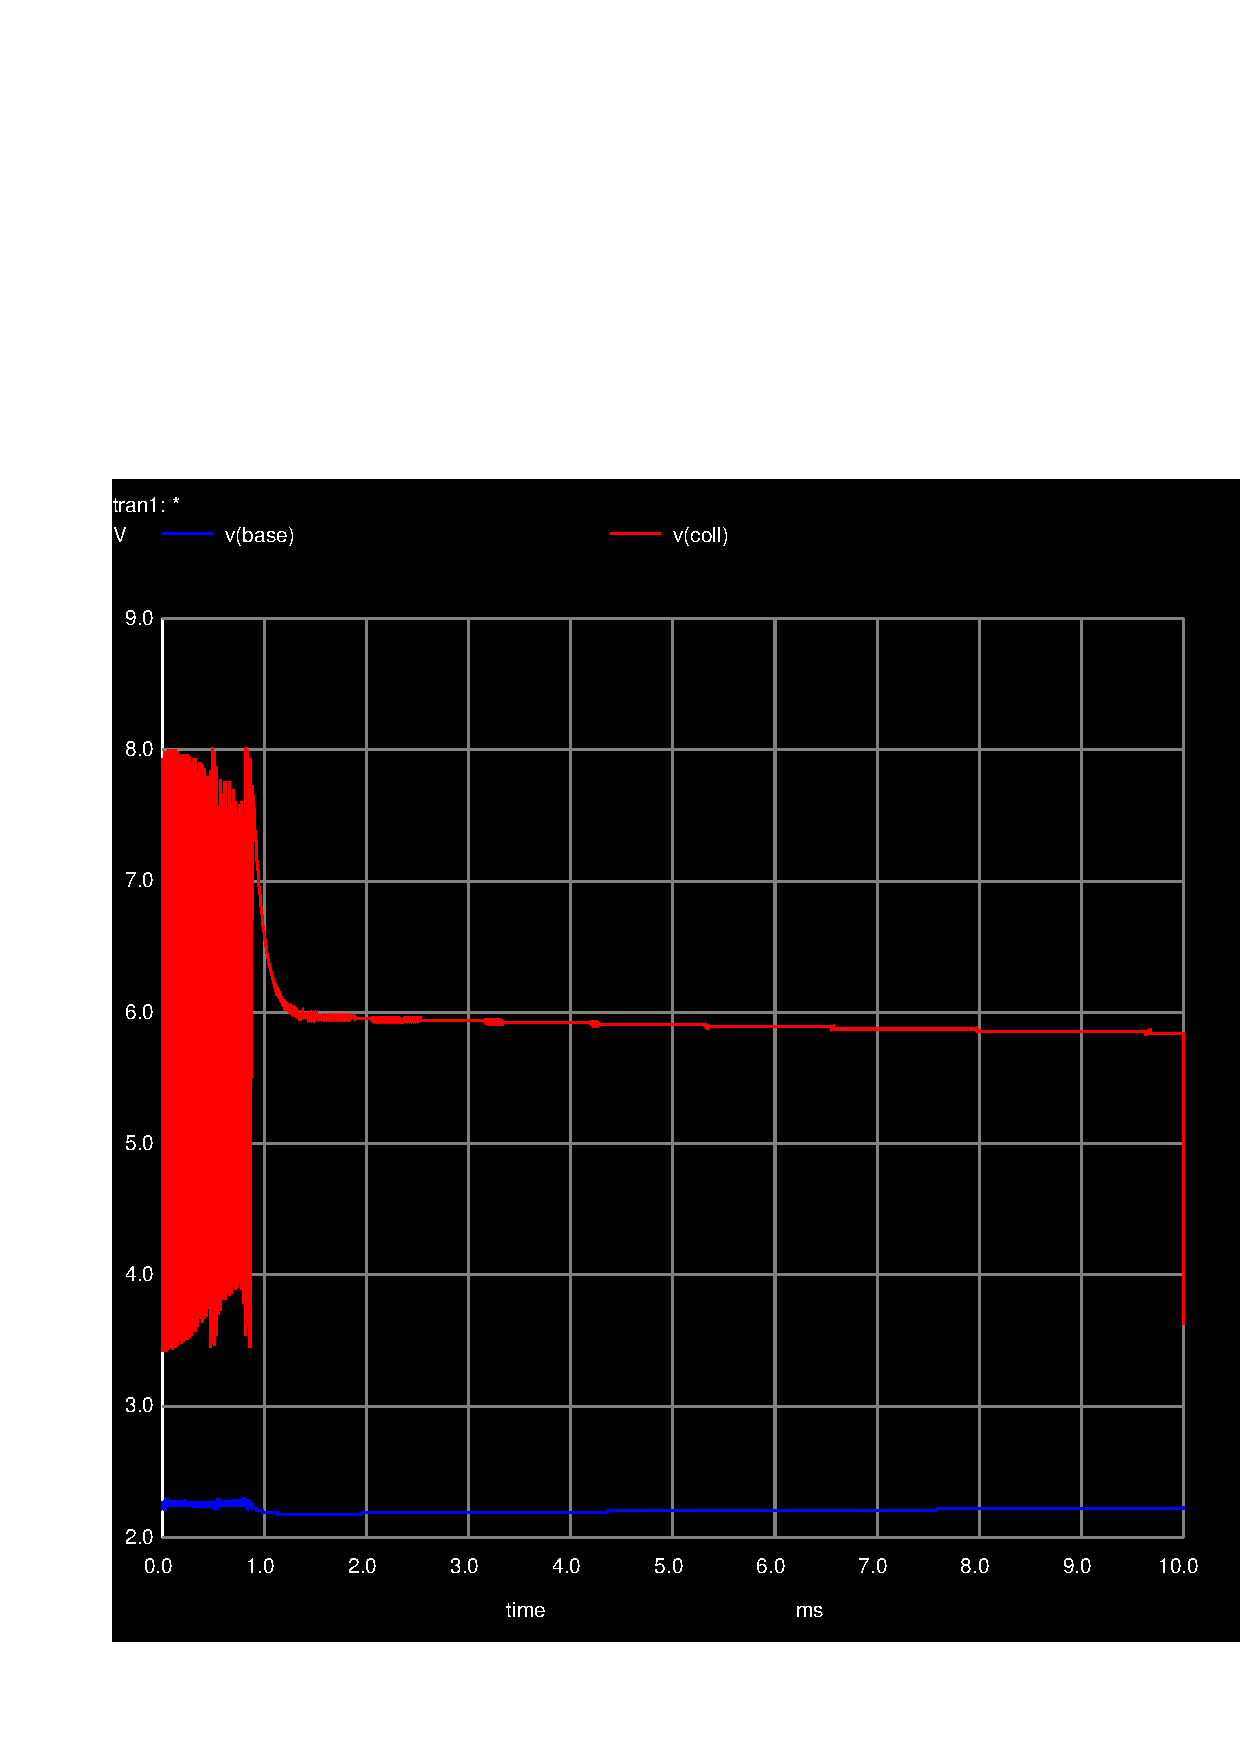
\includegraphics[width=0.6\linewidth]{trans.pdf}
\caption{Transient output voltage}
\label{fig:trans}
\end{figure}

\lipsum[1-1]



\subsection{Frequency Analysis}

\subsubsection{Magnitude Response}

Figure~\ref{fig:acm} shows the magnitude of the frequency response for the
circuit under analysis. Compared to the theoretical analysis results, one
notices the following differences: describe and explain the differences.

\begin{figure}[h] \centering
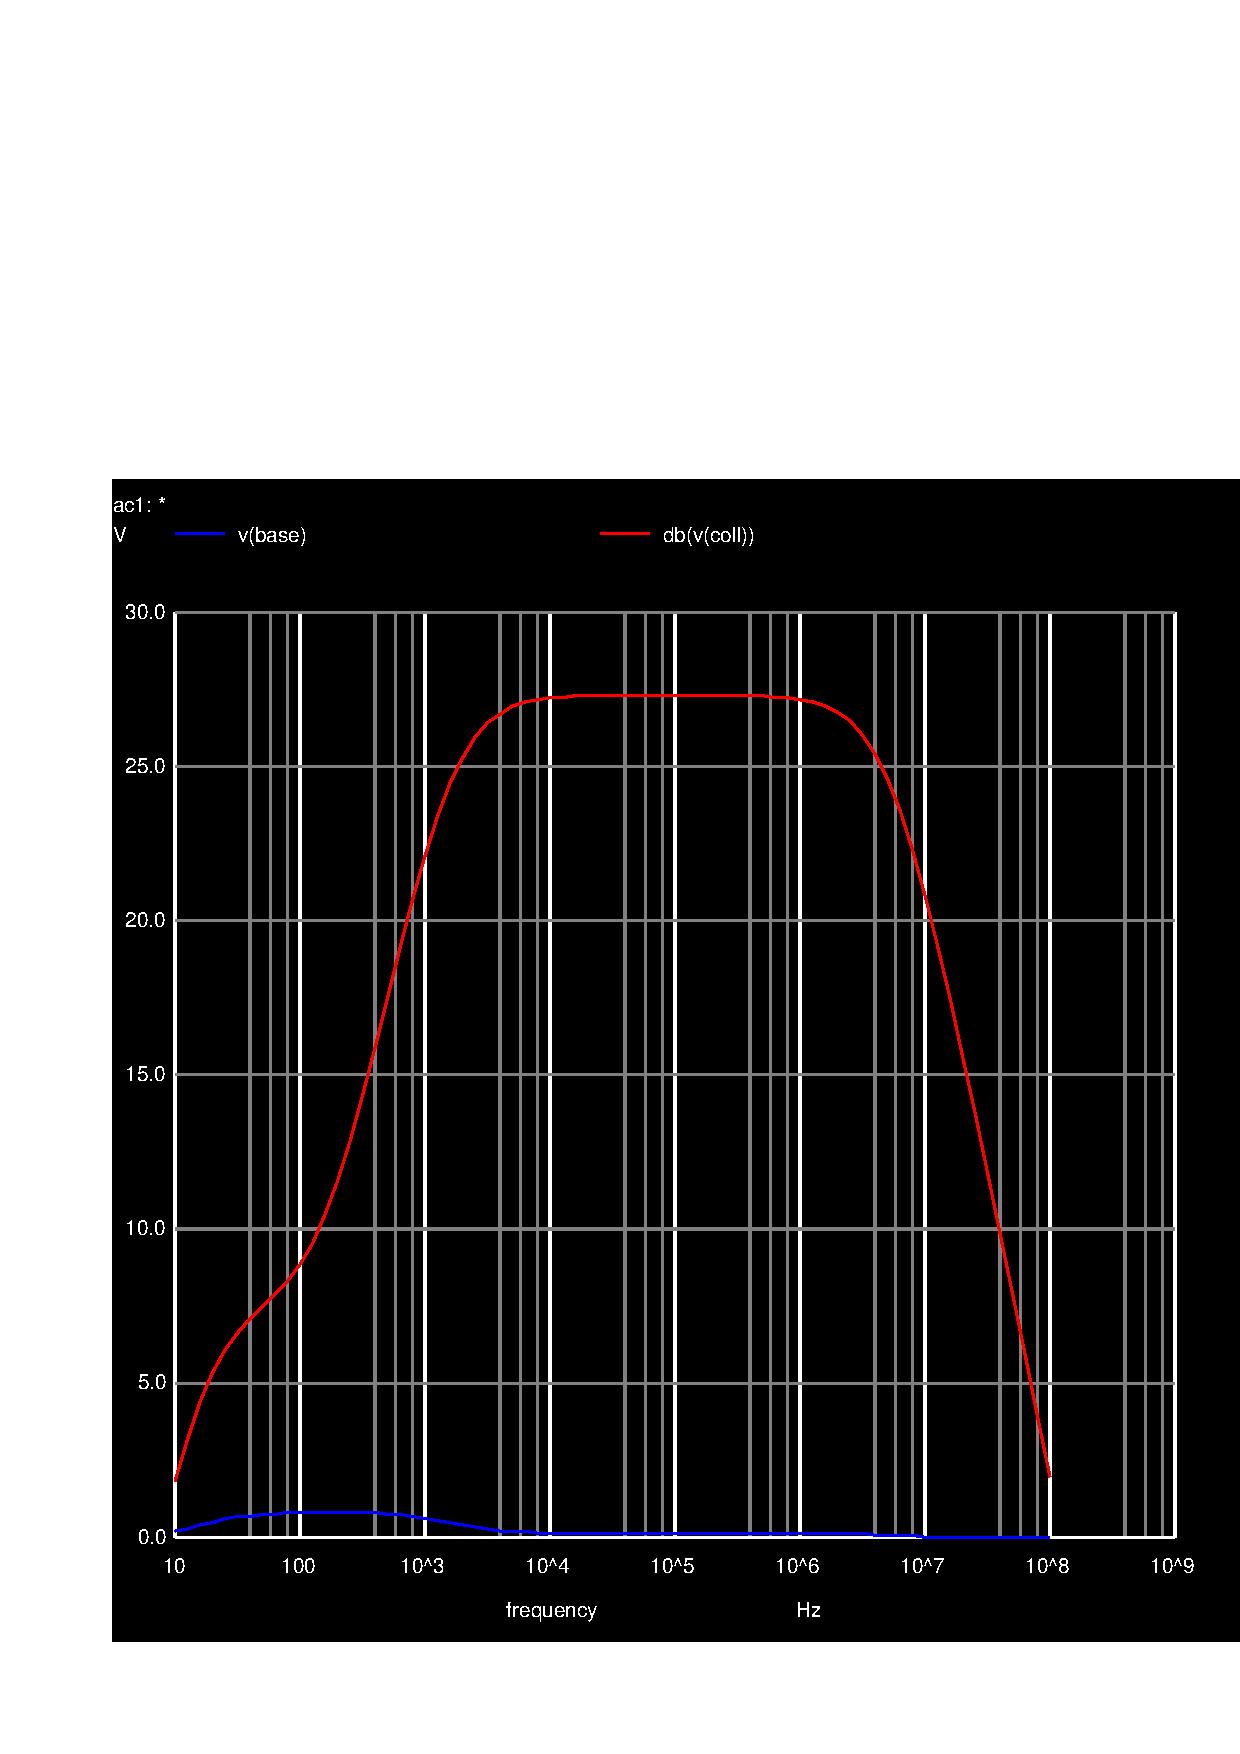
\includegraphics[width=0.6\linewidth]{acm.pdf}
\caption{Magnitude response}
\label{fig:acm}
\end{figure}

\lipsum[1-1]

\subsubsection{Phase Response}

Figure~\ref{fig:acp} shows the magnitude of the frequency response for the
circuit under analysis. Compared to the theoretical analysis results, one
notices the following differences: describe and explain the differences.

\begin{figure}[h] \centering
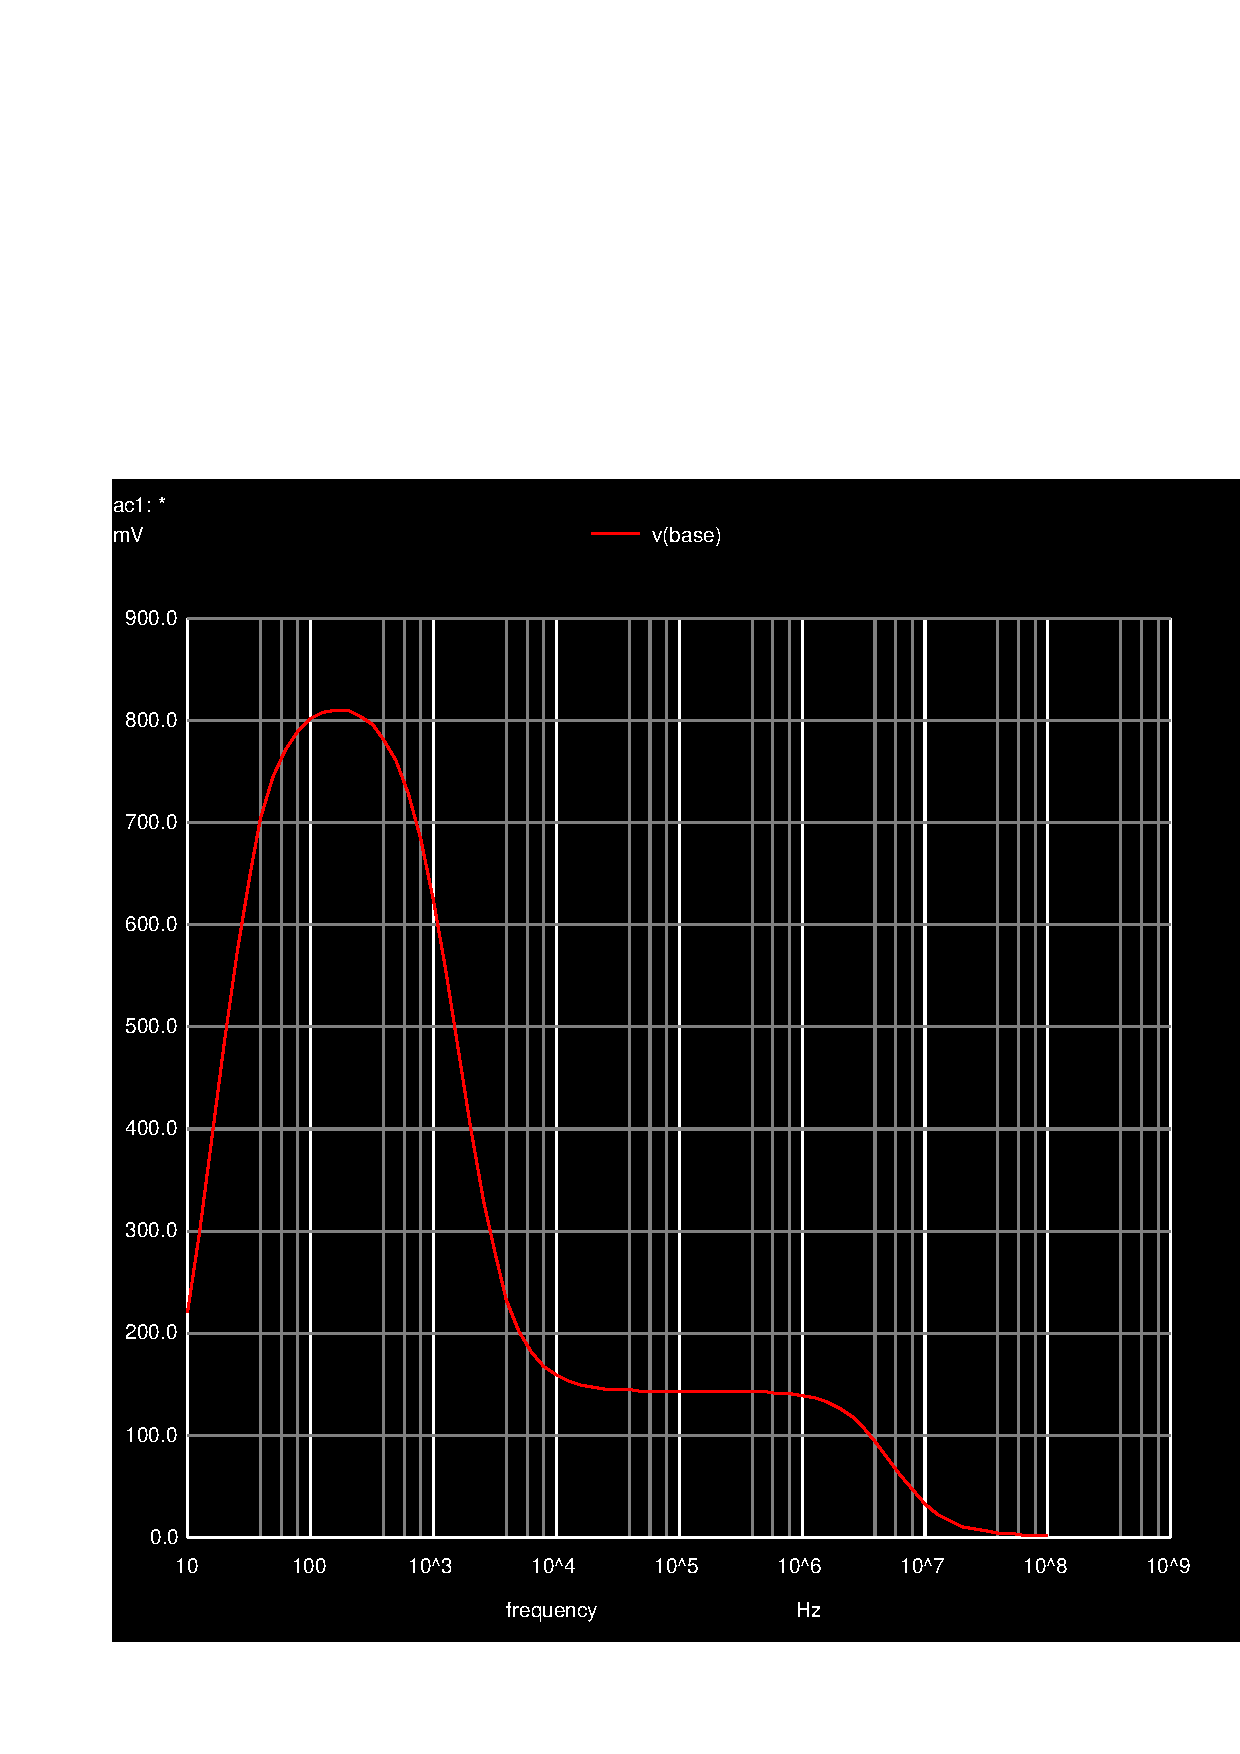
\includegraphics[width=0.6\linewidth]{acp.pdf}
\caption{Phase response}
\label{fig:acp}
\end{figure}

\lipsum[1-1]

\subsubsection{Input Impedance}

Figure~\ref{fig:zim} shows the magnitude of the frequency response for the
circuit under analysis. Compared to the theoretical analysis results, one
notices the following differences: describe and explain the differences.

\begin{figure}[h] \centering
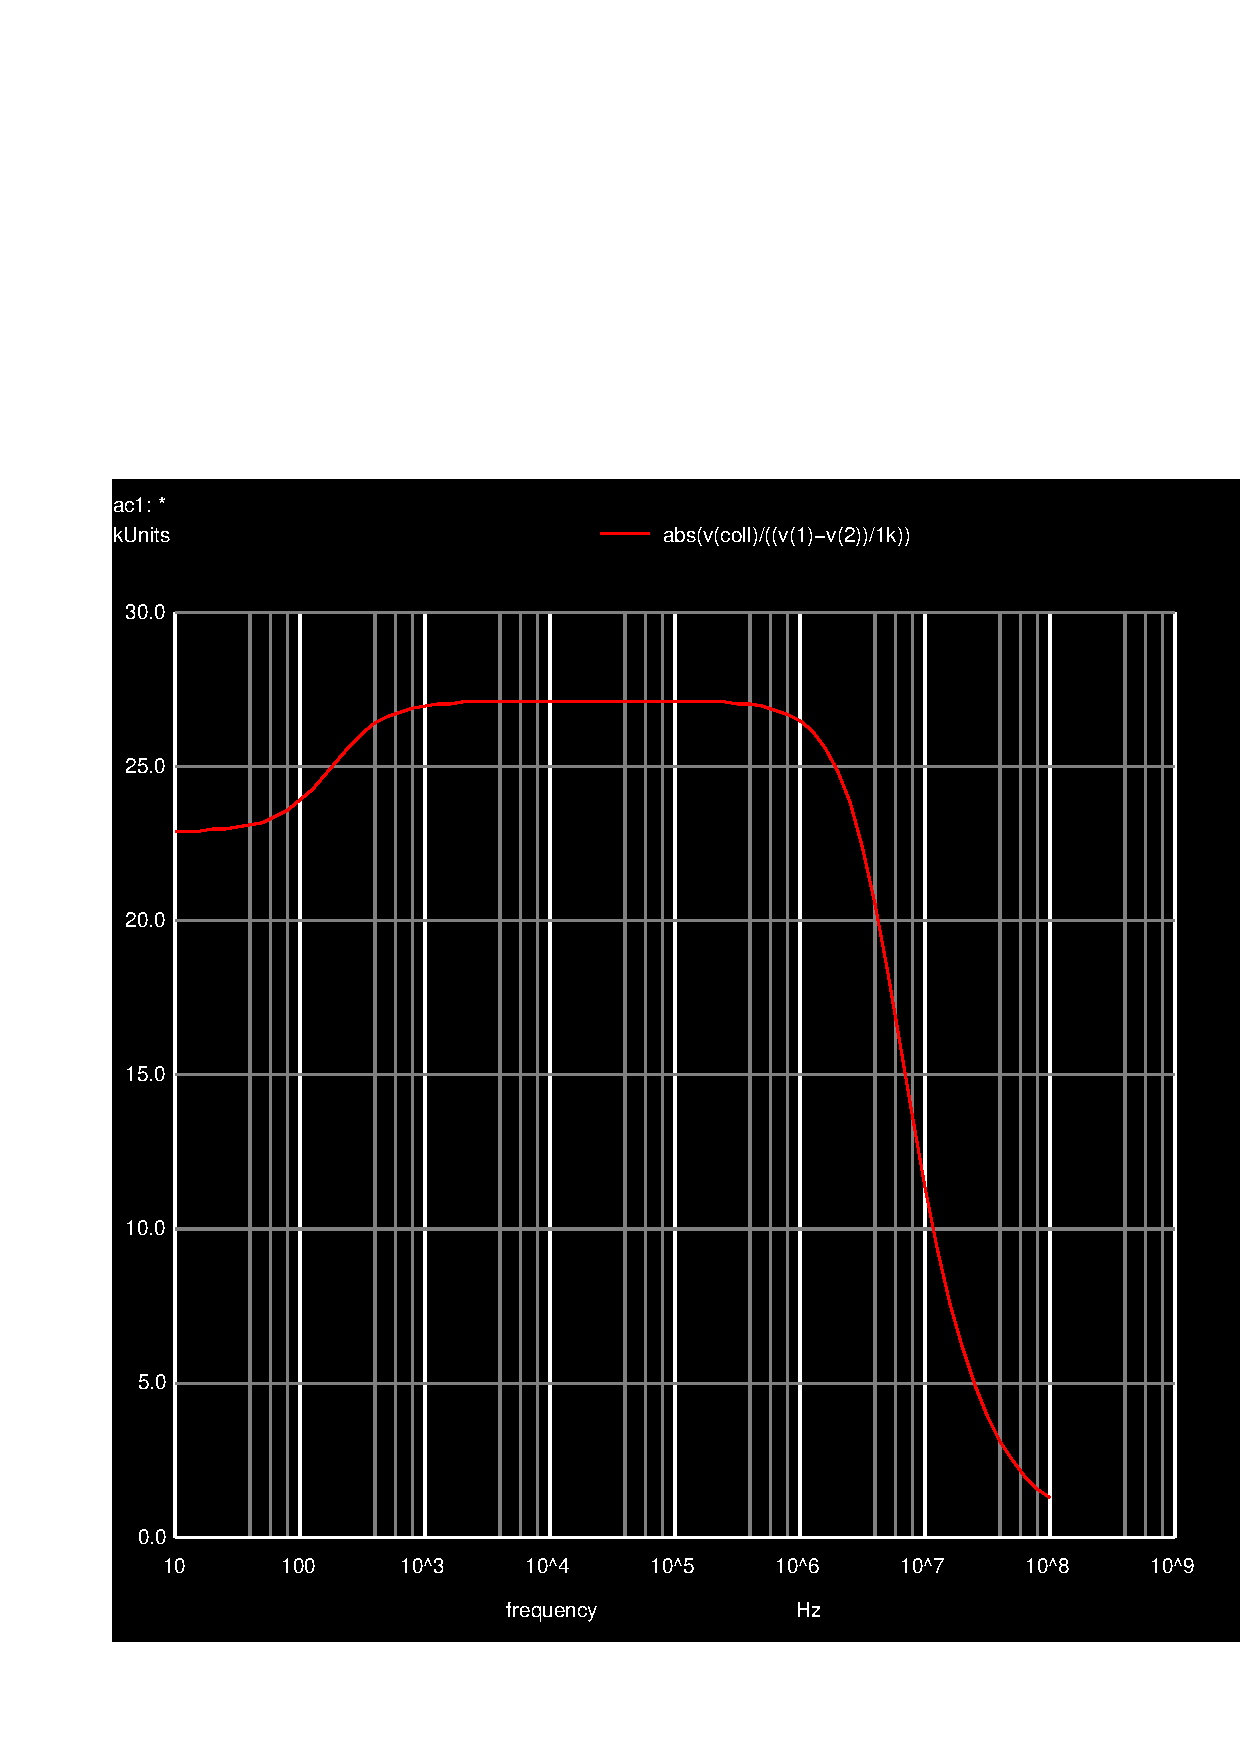
\includegraphics[width=0.6\linewidth]{zim.pdf}
\caption{Input impedance}
\label{fig:zim}
\end{figure}

\lipsum[1-1]






\section{Theoretical Analysis}
\label{sec:theoretical analysis}
%%%%%%%%%%%%%%%%%%%%%%%%%%%%%%%%%%%%%%%%%%%%%

\subsection{Results at Central Frequency}

\indent

Because this a band pass filter there is a lower cut off frequency, $f_L$ and a high cut off frequency, $f_H$. With these frequencies, we can define $\omega_L$ and $\omega_H$.

The former can be calculated like so,


\[\omega_L = \frac{1}{R_1 C_1}\tag{1}\label{1}\]

and the latter can be calculated like so, \[\omega_H = \frac{1}{R_2 C_2}\tag{2}\label{2}\]

The central frequency can then be obtained through the following formula: 

\[\omega _0 =\sqrt{\omega _L \omega _H}\tag{3}\label{3}\]

\vspace{0.5cm}
\begin{center}
\csvautotabular{../mat/resultados2.txt}
\csvautotabular{../sim/comp1.txt}
\end{center}

Despite nott being able to predict accurately the lower and higher cut off frequency, the central frequency can be predicted quite well. 

\vspace{1cm}

To compute gain of the circuit at the central frequency, the circuit was analysed in its three parts,  the high pass filter, the amplification stage and the low pass filter, resulting in the respective formulae:

\vspace{0.5cm}

\[gain_{HPF}=\frac{j\omega _0 R_1 C_1}{1+j \omega _0 R_1 C_1};\tag{4}\label{4}\]
 
\[gain_{Amplifier}=1+R_3/R_4;\tag{5}\label{5}\]
 
\[gain_{LPF} = \frac{1}{1+j \omega _0 R_2 C_2}.\tag{6}\label{6}\]
 
\vspace{1cm}
 
The gain can then be obtained by the multiplication of each of the previous gains.
 

 
\vspace{1cm}

In order to obtain the input and output impedances the following formulae were used:
\vspace{0.5cm}
 
\[Z_i = \frac{1}{j\omega _0 C_1} + R_1\tag{7}\label{7}\]
 
 \[Z_o = \frac{1}{1/R_2 + j \omega _0 C_2}\tag{8}\label{8}\]



\vspace{1cm}

This results in the following results:

\vspace{0.5cm}
\begin{center}
\csvautotabular{../mat/resultados.txt}
\csvautotabular{../sim/comp2.txt}
\end{center}
\vspace{1cm}

As it can be seen, the gain and input impedances have similar values, but the output impedance does not. This can be explained by the fact that the AM-POP is considered to be ideal in theoretical analysis, while in the simulation it acts like a real AM-POP.  

\subsection{Frequency Response}

\indent

The frequency response can be was obtained the same way as it was done with the gain, but by applying the formula to many frequencies. This way, the transfer function will be:

\vspace{0.5cm}

\[f_{res}=\frac{R_1 C_1 \omega j}{1 + R_1 C_1 \omega j}\times(1 + \frac{R_3}{R_4}) \times \frac{1}{1+ R_2 C_2 \omega j} \tag{9}\label{9}\]

\vspace{0.5cm}
With this function we can obtain the following plots:

\vspace{0.5cm}
% imagem1 

\begin{figure}[h]
    \centering
\subfloat[Simulation Results]{\includegraphics[width=0.40\textwidth]{../sim/vof.pdf}
\label{gain_sim}}
  \hfill
\subfloat[Theoretical Results]{\includegraphics[width=0.55\textwidth]{../mat/gain.png}
\label{gain_teo}}
\end{figure}

  \begin{figure}[h]
     \centering
     \caption{Gain}
     \label{gain}
 \end{figure}
 
\vspace{0.5cm}
 
 % imagem1 

\begin{figure}[H]
    \centering
\subfloat[Simulation Results]{\includegraphics[width=0.40\textwidth]{../sim/vop.pdf}
\label{phase_sim}}
  \hfill
\subfloat[Theoretical Results]{\includegraphics[width=0.55\textwidth]{../mat/phase.png}
\label{phase_teo}}
\end{figure}

  \begin{figure}[h]
     \centering
     \caption{Phase}
     \label{phase}
 \end{figure}
 
 
 \vspace{1cm}

By looking at the previous results, it is possible to see that the theoretical model can predict quite well the value of the gain given a certain frequency. However, the same can't be said about the phase plots. Although, they start similar, as the frequencies get bigger, the results become completely differet.

This way, the merit will be

\begin{table}[H]
  \centering
  \begin{tabular}{|l|r|}
    \hline    
    %{\bf Name} & {\bf Value [A or V]} \\ \hline
    \input{../mat/merito.txt}
  \end{tabular}
  \caption{Theoretical M}
  \label{tab:M_T}
\end{table}

\begin{table}[H]
  \centering
  \begin{tabular}{|l|r|}
    \hline    
    %{\bf Name} & {\bf Value [A or V]} \\ \hline
    \input{../sim/comp3.txt}
  \end{tabular}
  \caption{Simulation M}
  \label{tab:M_S}
\end{table}

Even with the previous mistakes, the theoretical analysis yields a decent estimate for the merit value with a similar order of magnitude.




\section{Conclusion}
\label{sec:conclusion}


\par Unlike previous laboratories, this time, the results were not equal.

However, we believe that the differences are not that significant and they can be explained by how NGSpice solves the circuit compared to how it was done in the theoretical analysis.

To solve the circuit, NGSpice used far more advanced simulation methods for the diodes, with many more parameters, while we used an approximated model with $V_{on}$ and an incremental resistor. 

This way, the objective should have never been to have equal results, but rather, have results that are "close enough", which we believe it was achieved.


%To sum up, we believe that the goals of this report were achieved.


%\cleardoublepage

% ----------------------------------------------------------------------
%  Bibliography
% ----------------------------------------------------------------------
%\addcontentsline{toc}{section}{\bibname}
%\bibliographystyle{abbrvunsrtnat} % <<<<< SELECT IF USING REFERENCES BY NUMBER (CITATION ORDER)
%\bibliography{../../../BIBfile.bib}

% ----------------------------------------------------------------------
\end{document}
% ----------------------------------------------------------------------
